\documentclass[10pt,a4paper]{article}
\usepackage[utf8]{inputenc}
\usepackage[czech]{babel}
\usepackage[T1]{fontenc}
\usepackage{epsfig}
\usepackage{fullpage}
\usepackage{listings}
\usepackage{color}
\usepackage{hyperref}
\usepackage{ amssymb }
\usepackage{ mathrsfs }
\usepackage{amsthm}
\usepackage{amsmath}
\usepackage{amsfonts}
\newtheorem{veta}{Věta}
\newtheorem{definition}{Definice}
\newtheorem{note}{Poznámka}




\begin{document}

\title{Státnicový okruh 4: \\ Informační technologie}
\maketitle
\newpage
\tableofcontents
\newpage

%-----------------------------------prvni odstavec------------------------------------
\section{}
\paragraph{John von Neumannova a harvardská architektura počítače, princip jeho činnosti. Binární logika, logické operace a funkce, logické obvody. Reprezentace čísel a znaků v paměti počítače. Osobní počítač (PC), základní deska, chipset a sběrnice (interní, externí). Procesor (CPU), vykonávání instrukcí, podprogramy a zásobník, přerušení. Paměti počítače (RAM, cache, disk, diskové pole). Přídavné karty PC, datové mechaniky a média (CD, DVD, paměťové karty), periferie.}



\newpage
%-----------------------------------druhy odstavec------------------------------------
\section{}
\paragraph{Operační systém, architektura, poskytovaná rozhraní. Správa procesoru: procesy a vlákna, plánování jejich
běhu, komunikace a synchronizace. Problém uváznutí, jeho detekce a metody předcházení. Správa operační pa-
měti: segmentace, stránkování, virtuální paměť. Správa diskového prostoru: oddíly, souborové systémy, zajištění
konzistence dat.}




\newpage
%-----------------------------------treti odstavec------------------------------------
\section{}
\paragraph{Klasifikace (LAN/MAN/WAN) a služby počítačových sítí. Síťová architektura TCP/IP a referenční model
ISO OSI. Strukturovaná kabeláž, přepínaný Ethernet a WLAN. Protokol IP, adresa a maska, směrování, IP
multicast. Protokoly TCP a UDP, správa spojení a řízení toku dat. Systém DNS, překlad jména (na IP adresu,
reverzní), protokol. Služby WWW, elektronické pošty, přenosu souborů a vzdáleného přihlášení.}
\paragraph{POZOR!} packet = jakákoliv naformátovaná zpráva jako packet vs. datagram = packet nespolehlivého přenosu dat.
\subsection{Klasifikace (LAN/MAN/WAN)}
Klasifikace sítí podle různých kritérií: rozlehlost, rychlost přenosu (klasické, vysokorychlostní), forma aplikace, dělení podle postavení uzlů (perr-to-peer, klient-server), podle druhu přenášení signálů (analog vs. digital) aj.
\subsubsection{Dělení podle rozlehlosti}
\begin{itemize}
	\item \textbf{PAN (Personal Area Network)}: Sítě s nejmenší rozlehlostí. Propojení mobilů, PDA, atd. Požadavky na odolnost vůči rušení, nízká spotřeba energie, snadná implementace.Ppřenosová rychlost není prioritou (zpravidla jen několik Mb/s). Dosah pouze několik metrů. Typické technologie Bluetooth, IrDA, Wifi.
	\item \textbf{LAN (Local Area Network)}: Sítě propojující koncové uzly typu počítač, tiskárna, server. V soukromé správě, dosah jednotky km (v rámci budovy/komplexu budov). Přenosové rychlosti 10Mb/s až 1Gb/s. Sdílené využití přenosového média. Ethernet, Wifi.
	\item \textbf{MAN (Metropolitan Area Network)}: Propojení několika LAN (účelem přenosové sítě, charakterem lokální). V rámci města (desítky km). Přenosové rychlosti jak vyšší (několik Gb/s), tak i nižší (<1Gb/s) ve srovnání s LAN.
	\item \textbf{WAN (Wide Area Network)}: Rozsáhlé sítě spojující LAN/MAN (páteřní sítě, telekomunikační - broadband). Velké vzdálenosti (prakticky neomezené). Mohou být soukromé i veřejné. Vysoké přenosové rychlosti (až stovky Gb/s). Příklad GPRS, xDSL, aj. Pronájem kapacity sítě = vyhrazené nesdílené využití přenosového média.
\end{itemize}
\subsubsection{Dělení podle topologie}
Topologie počítačové sítě říká, jak jsou vlastně prvky v této síti uspořádány.
\paragraph{Kruhová topologie (RING)}
Každý počítač je propojen přímo s předchozím a následujícím počítačem v kruhu. V LAN je používána velmi málo, používá se v průmyslových sítí nebo sítích MAN. \\ Výhody:
\begin{itemize}
	\item lehce rozšiřitelná struktura
	\item malý počet spojů
	\item snadné vysílání, zprávy v kruhu od stanice ke stanici
\end{itemize}
Nevýhody:
\begin{itemize}
	\item výpadek libovolné stanice zapříčiní výpadek celé sítě, úplný výpadek sítě při přerušení kabelu v  libovolném místě
	\item poměrně veliké nebezpeční odposlechu síťové komunikace, která prochází přes spojovací počítače
\end{itemize}
Problém výpadku se řešil tzv. dvojitým kruhem, ve kterém byly stanice propojeny dvěma kruhy, každý v opačné směru.
\paragraph{Sběrnicová topologie (BUS)}
Tato topologie patří k nejstarším, všechny stanice jsou připojeny na pasivní společné médium, které sdílejí. Dnes už se tato topologie příliš nepoužívá, ale na začátku devadesátých let byla dominantní. Tím společným médiem byl koaxiální kabel, pomocí kterého se jednotlivé počítače připojily do sítě. \\
Výhody:
\begin{itemize}
	\item nezávislost stanic na výpadku libovolné jiné stanice
	\item levné náklady takového řešení
	\item neexistence aktivních prvků
	\item snadné všesměrové vysílání
\end{itemize}
Nevýhody:
\begin{itemize}
	\item úplný výpadek sítě při přerušení kabelu v libovolném místě
	\item nutnost vyřešení přístupu stanic k médiu (kdo bude vysílat)
\end{itemize}
Výhody a nevýhody jsou relativní a poplatné době. To, že se v dobách používání této topologie v sítích LAN, považovala absence aktivních prvků za výhodu, bychom v dnešní době řadili spíše k nevýhodě.
\paragraph{Hvězdicová topologie}
Tato topologie je dnes jednoznačně nejpoužívanější topologií v sítích LAN. Myšlenka spočívá v tom, že existuje centrální prvek, který spojuje všechny prvky. Dříve tím centrálním prvkem býval počítač, dnes je aktivní prvek (HUB nebo SWITCH). \\
Výhody:
\begin{itemize}
	\item lehce rozšiřitelná struktura
	\item výpadek libovolné stanice neznamená výpadek celé sítě
	\item větší možnosti zabezpečení, při použití aktivních prvků typu SWITCH je většina síťové komunikace skryta před ostatními účastníky sítě
\end{itemize}
Nevýhody:
\begin{itemize}
	\item nutnost použití hubu nebo switche
	\item vyžaduje veliké množství kabelů a je tak náročná na montáž
\end{itemize}
\paragraph{Páteřní topologie}
Páteřní topologií rozumíme situaci, kdy pomocí určité topologie propojujeme celé sítě LAN. Páteřní topologie může být zapojena jako sběrnice, hvězda i kruh, často se používá zapojení typu kruh. Jejím základem je vytvoření nezávislé hlavní části, která propojuje důležité celky. Na ni se naopak připojují různé subsítě nebo segmenty. V případě výpadku libovolného segmentu zůstává provoz na páteři neohrožen. Páteř může mít vyšší přenosovou rychlost.
\subsubsection{Služby počítačových sítí}
\begin{itemize}
	\item připojení k síti
	\item vzdálený přístup, sdílení výpočetních prostředků a přenos dat (sdílené databáze, perr-to-peer sítě, sdílené soubory)
	\item sdílení technických prostředků (tiskárny, faxy, disky, apod.)
	\item adresářové služby (jednotný přístup do informačního systému a k informacím z centrální databáze, např. LDAP, Active Directory)
	\item elektronická pošta a výměna dokumentů (objednávky, faktury, atd.)
	\item online komunikace/multimedia (např. IRC, VoIP, straming, hry) - vysoké nároky na síť
	\item informační služby, internetové aplikace (WWW, business a desktopové aplikace)
	\item monitorování a vzdálená administrace sítě
\end{itemize}
Komunikace uzlů a propojovacích prvků sítě na různých úrovních:
\begin{itemize}
	\item nižší - přenos bloků dat, většinou nespolehlivý (bez potvrzení a opakování přenosu), nespojová komunikace
	\begin{itemize}
		\item \textbf{unicast}: dvoubodová, základní
		\item \textbf{multicast}: bod-skupina, např. straming, virtuální sítě
		\item \textbf{broadcast}: bod-všichni, např. konfigurace a zapojení do sítě
	\end{itemize}
	\item vyšší - komunikace aplikací, většinou spolehlivá (s potvrzením doručení, popř. opakování přenosu), spojově orientovaná (vytvořeno spojení mezi aplikacemi)
	\begin{itemize}
		\item \textbf{peer-to-peer}: zpravidla rovnocenná výměna dat
		\item \textbf{klient-server}: hiearchická, forma požadavek-odpověď
	\end{itemize}
\end{itemize}
Typy koncových uzlů:
\begin{itemize}
	\item \textbf{pracovní stanice} (work station, klient): převážně využívá služeb sítě
	\begin{itemize}
		\item \textbf{tenký klient}: znakový/grafický HW terminál, pouze zprostředkování vstupu a výstupu pro vzdálený server, nemůže pracovat samostatně
		\item \textbf{tlustý klient}: osobní počítač - klientské části síťových služeb i lokální úlohy, může (do určité míry) fungovat samostatně
	\end{itemize}
	\item \textbf{server}: převážně poskytuje služby v síti \\ souborový (FTP, NFS, SMB), databázový/adresářový (SŘBD, LDAP), poštovní (IMAP, POP3, SMTP), terminálový (telnet, SSH), informační/WWW (HTTP), komunikační (IM, VoIP), tiskový, aj.
\end{itemize}




\subsection{Síťová architektura TCP/IP a referenční model ISO OSI.}
Snaha o vytvoření univerzálního konceptu sítě (topologie, formy a pravidlakomunikace, poskytování služeb atd.). Požadavky: decentralizace služeb, rozumná adresace uzlů, data zasílána v nezávislých blocích, směrování bloků, zabezpečení, kontrola a řízení přenosu aj. Dříve proprietární uzavřená řešení, následně standatdizace s koncepcí komunikace nezávislé na implementaci. \\
\textbf{Komunikace ve vrstvách}
\begin{itemize}
	\item definované službami poskytované vyšším vrstvám a využívající služby nižších vrstev, implementace skryté okolním vrstvám
	\item samostatné vrstvy s funkcemi podobnými v rámci vrstvy a odlišnými v různých vrstvách, nezávislé na implementaci
\end{itemize}
Komunikace mezi vrstvami pomocí \textbf{mezivrstvových protokolů} - na každé komunikující straně zvlášť; skrze \textbf{programová rozhraní}; prostřednictvím přístupových bodů; využívající tzv. služební primitiva.
\paragraph{Obecná služební primitiva}
\begin{itemize}
	\item žádost o službu (request)
	\item oznámení poskytovatele o přijetí žádosti (indication) - nepovinné
	\item odezva poskytovatele (response), příp. vytvoření spojení
	\item potvrzení odezvy žadatelem (confirmation) - nepovinné
\end{itemize}
Komunikace ve stejných vrstvách mezi entitami (zařízeními) pomocí \textbf{vrstvových protokolů}.
\subsubsection{Protokol}
= souhrn pravidel (norem a doporučení) a procedur pro komunikaci (výměnu dat). Obsahuje syntaktická a sémantická pravidla výměny protokolových datových jednotek.\\
\textbf{Protokolové datové jednotky} = režijní informace a data (rámce, pakety, segmenty). Komunikace zprostředkována sousední nižší vrstvou. Na straně odesílatele \textbf{zapouzdřování} od nejvyšší po nejnižší vrstvu. Na straně příjemce \textbf{rozbalování} dat v opačném směru.
\paragraph{Síťová (protokolová) architektura} = definice vrstev, služeb funkcí, protokolů a forem komunikace. Normalizované (OSI, TCP/IP) a firemní proprietární (Novell NetWare, SMB, Apple Appletalk aj.)
\paragraph{Abstraktní referenční síťový model} Abstrakce konkrétních síťových architektur - nemusí podporovat všechny funkce modelu (např. průmyslové sítě nepodporují směrování, propojení pomocí mostů a bran).
\subsubsection{Referenční model ISO/OSI}
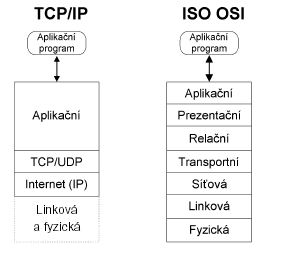
\includegraphics[width=8cm]{img/modely.png} \\
Propojení otevřených systémů = zařízení podporující příslušné normy. Deinovány koncové uzly (koncová datová zařízení) a mezilehlé uzly (propojovací prvky). \\
Každá ze sedmi vrstev vykonává skupinu jasně definovaných funkcí potřebných pro komunikaci. Pro svou činnost využívá služeb své sousední nižší vrstvy. Své služby pak poskytuje sousední vyšší vrstvě. Podle referenčního modelu není dovoleno vynechávat vrstvy, ale některá vrstva nemusí být aktivní. Takové vrstvě se říká nulová, nebo transparentní. \\
Na počátku vznikne požadavek některého procesu v aplikační vrstvě. Příslušný podsystém požádá o vytvoření spojení prezentační vrstvu. V rámci aplikační vrstvy je komunikace s protějším systémem řízena aplikačním protokolem. Podsystémy v prezentační vrstvě se dorozumívají prezentačním protokolem. Takto se postupuje stále níže až k fyzické vrstvě, kde se použije pro spojení přenosové prostředí. Současně se při přechodu z vyšší vrstvy k nižší přidávají k uživatelským (aplikačním) datům záhlaví jednotlivých vrstev. Tak dochází k postupnému zapouzdřování původní informace. U příjemce se postupně zpracovávají řídící informace jednotlivých vrstev a vykonávají jejich funkce.
\paragraph{Fyzická vrstva} Specifikuje fyzickou komunikaci. Aktivuje, udržuje a deaktivuje fyzické spoje mezi koncovými systémy. Definuje všechny elektrické a fyzikální vlastnosti zařízení (tvary konektorů; typy médií = kroucená dvojlinka, optické vlákno, mikrovlny; přenosové rychlosti). Obsahuje rozložení pinů, napěťové úrovně a specifikuje vlastnosti kabelů. \\
Funkce poskytované fyzickou vrstvou:
\begin{itemize}
	\item Navazování a ukončování spojení s komunikačním médiem.
	\item Spolupráce na efektivním rozložení všech zdrojů mezi všechny uživatele.
	\item Modulace neboli konverze digitálních dat na signály používané přenosovým médiem (a zpět) (A/D, D/A převodníky).
\end{itemize}
HW zařízení: HUB, opakovač.
\paragraph{Linková vrstva} Poskytuje spojení mezi dvěma sousedními systémy. Uspořádává data z fyzické vrstvy do logických celků = \textbf{rámce (frames)}: záhlaví s linkovou adresou příjemce a odesílatele (např. MAC) + data + zápatí s kontrolním součtem (CRC) celého rámce. Stará se o nastavení parametrů přenosu linky, oznamuje neopravitelné chyby. Formátuje fyzické rámce, opatřuje je fyzickou adresou a poskytuje synchronizaci pro fyzickou vrstvu. Příkladem je MAC u Ethernetu. Poskytuje propojení pouze mezi místně připojenými zařízeními a tak vytváří doménu na druhé vrstvě pro směrové a všesměrové vysílání. \\
HW zařízení: most, přepínač, síťová karta, přístupový bod.
\paragraph{Síťová vrstva} Stará se o směrování v síti a síťové adresování. Poskytuje spojení mezi systémy, které spolu přímo nesousedí. Poskytuje funkce k zajištění přenosu dat různé délky od zdroje k příjemci skrze jednu případně několik vzájemně propojených sítí při zachování kvality služby, kterou požaduje přenosová vrstva. Síťová vrstva poskytuje směrovací funkce a také reportuje o problémech při doručování dat. Jednotkou přenosu je \textbf{síťový packet}: záhlaví se síťovou adresou příjemce a odesílatele (např. IP) + data + zápatí jen výjimečně. \\
Funkce poskytované síťovou vrstvou:
\begin{itemize}
	\item abstrakce různých linkových technologií
	\item správa linkových spojení, multiplexování síťových spojení do linkových (více datových toků kombinováno do jednoho)
	\item formátování dat do packetů
	\item směrování packetů
	\item zjišťování a oprava chyb
	\item vytváření podsítí
\end{itemize}
HW zařízení: směrovač, brána.
\paragraph{Transportní vrstva} Zajišťuje přenos dat mezi koncovými uzly. Jejím účelem je poskytnout takovou kvalitu přenosu, jakou požadují vyšší vrstvy. Vrstva nabízí spojově (TCP) a nespojově orientované (UDP) protokoly. Jednotkou přenosu je \textbf{transportní packet}: záhlaví s transportní adresou příjemce a odesílatele + data. \\
\textbf{TCP}: Protokol garantuje spolehlivé doručování a doručování ve správném pořadí. TCP také umožňuje rozlišovat a rozdělovat data pro více aplikací (například webový server a emailový server) běžících na stejném počítači. TCP využívá mnoho populárních aplikačních protokolů a aplikací na internetu, včetně WWW, e-mailu a SSH. \\
\textbf{UDP}: Na rozdíl od protokolu TCP nezaručuje, zda se přenášený datagram neztratí, zda se nezmění pořadí doručených datagramů, nebo zda některý datagram nebude doručen vícekrát. UDP je vhodný pro nasazení, které vyžaduje jednoduchost nebo pro aplikace pracující systémem otázka-odpověď (např. DNS, sdílení souborů v LAN). \\
Funkce poskytované transportní vrstvou:
\begin{itemize}
	\item adresování (transportní na síťové)
	\item správa síťových spojení
	\item multiplexování a větvení
	\item rozdělení dat na datagramy, segmentace, formátování
	\item řízení proudu dat (správné pořadí datagramů), optimalizace služeb
	\item koncová detekce a oprava chyb
\end{itemize}
Umožňuje \textbf{duplexní přenos} (= přenos oběma směry).
\paragraph{Relační vrstva} Smyslem vrstvy je organizovat a synchronizovat dialog mezi spolupracujícími relačními vrstvami obou systémů a řídit výměnu dat mezi nimi (např. sdílení síťového disku). Umožňuje vytvoření a ukončení relačního spojení, synchronizaci a obnovení spojení, oznamovaní výjimečných stavů. Jednotka přenosu je \textbf{relační packet}: poze data. \\
Funkce poskytované relační vrstvou:
\begin{itemize}
	\item organizace a synchronizcae dialogu výměny dat (pomocí kontrolních bodů)
	\item zobrazení relačních spojení do transportních
	\item správa transportních spojení
\end{itemize}
\paragraph{Prezentační vrstva} Funkcí vrstvy je transformovat data do tvaru, který používají aplikace (šifrování, konvertování, komprimace). Formát dat (datové struktury) se může lišit na obou komunikujících systémech, navíc dochází k transformaci pro účel přenosu dat nižšími vrstvami. Vrstva se zabývá jen strukturou dat, ale ne jejich významem, který je znám jen vrstvě aplikační. \\
Funkce poskytované prezentační vrstvou:
\begin{itemize}
	\item transformace a výběr reprezentace dat
	\item formátování, komprese, zabezpečení (šifrování), integrita dat
	\item transparentní přenos zpráv (nezná jejich význam
\end{itemize}
\paragraph{Aplikační vrstva} Účelem vrstvy je poskytnout aplikacím přístup ke komunikačnímu systému a umožnit tak jejich spolupráci. \\
Funkce poskytované aplikační vrstvou:
\begin{itemize}
	\item zprostředkování funkcionality sítě
	\item přenos zpráv, určení kvality, synchronizace
	\item identifikace, stanovení pověření
	\item dohoda o ochraně, o opravách chyb
\end{itemize}
Protokoly: SMTP, SSH, Telnet, POP3, DHCP, FTP, DNS aj.
\paragraph{Funkce společné více  vrstvám}
Komunikace \textbf{se spojením} má 3 fáze: navázání spojení, přenos dat, ukončení spojení. Dohoda na parametrech, použití potvrzování přijetí/nepříjetí (spolehlivost), stejné pořadí dat na vstupu i výstupu. \\
Komunikace \textbf{bez spojení}: při každém přenosu všechny parametry, nezávislý přenos datových jednotek, různé pořadí na vstupu a výstupu, spolehlivost i nespolehlivost. \\
Dále se může mezi těmito typy konvertovat. Transportní služby musí být se spojením.
\subsubsection{TCP/IP}
použití v síti Internet, nejpoužívanější síťová architektura. Síť tvořena směrovači, specializovanými bránami (bezpečnostní, aplikační, telekomunikační), lokálními sítěmi a koncovými zařízeními. Vlastní protokoly.
\paragraph{Vrstva síťového rozhraní} Nejnižší vrstva umožňuje přístup k fyzickému přenosovému médiu. Je specifická pro každou síť v závislosti na její implementaci.
\paragraph{Síťová vrstva} Vrstva zajišťuje především síťovou adresaci, směrování a předávání datagramů.
\paragraph{Transportní vrstva} je implementována až v koncových zařízeních (počítačích) a umožňuje proto přizpůsobit chování sítě potřebám aplikace. Poskytuje transportní služby kontrolovaným spojením spolehlivým protokolem TCP nebo nekontrolovaným spojením nespolehlivým protokolem UDP.
\paragraph{Aplikační vrstva} Vrstva aplikací. To jsou programy (procesy), které využívají přenosu dat po síti ke konkrétním službám pro uživatele. \\
Aplikační protokoly používají vždy jednu ze dvou základních služeb transportní vrstvy: TCP nebo UDP, případně obě dvě (např. DNS). Pro rozlišení aplikačních protokolů se používají tzv. porty, což jsou domluvená číselná označení aplikací. Každé síťové spojení aplikace je jednoznačně určeno číslem portu a transportním protokolem (a samozřejmě adresou počítače).
\subsubsection{Bezpečnost}
Obecné metody ochrany:
\begin{itemize}
	\item omezování přenosu dat a přístupu k síti: blokace, filtrace
	\item autorizace přístupu: jméno a heslo, vícefaktorové, speciální protokoly
	\item zabezpečení kanálu: šifrování, výměna klíčů
	\item autenticita zpráv: digitální podpis, certifikáty
\end{itemize}
\paragraph{TCP/IP} původně žádné zabezpečení, ponecháno na aplikaci. \\
Útoky:
\begin{itemize}
	\item falešná adresace (spoofing)
	\item analýza hesla, trojský kůň
	\item odposlech
	\item odmítnutí služby (DoS, zahlcení, vyčerpání zdrojů)
	\item zneužití chyb aplikací
	\item ...
\end{itemize}
Ochrana:
\begin{itemize}
	\item firewall (oddělení vnitřní sítě od vnější)
	\item překlad adres (NAT) - vlastní skrytá adresace
	\item aplikační brány (proxy)
	\item autentizace komunikujících stran
	\item zabezpečení komunikace (šifrování)
	\item opatření proti zahlcení
	\item ...
\end{itemize}




\subsection{Strukturovaná kabeláž, přepínaný ethernet a WLAN}
\subsubsection{Strukturovaná kabeláž}
Obecný pojem pro metalické a optické prvky, které umožňují propojení.
\paragraph{Telekomunikační přípojky} Slouží pro připojení koncových uživatelských zařízení - např. stolní počítač, notebook, analogový nebo ISDN telefon, VoIP telefon či síťová tiskárna. Telekomunikační zásuvky bývají umístěny přímo v pracovních prostorách (např. kancelářích) každé budovy, a to buď přímo ve zdi, v parapetních žlabech, případně podlahových systémech tak, aby byly lehce dostupné.
\paragraph{Patch panely} Na rozdíl od běžně dostupných zásuvek jsou patch panely umístěny v rozvaděčích v telekomunikační místnosti a nejsou tedy pro běžné uživatele přístupné. Patch panely slouží správci sítě k připojení jednotlivých uživatelů do aktivních zařízení jako jsou switche nebo telefonní ústředny. Pro připojení vodičů do zářezových konektorů se používá narážecí nástroj.
\paragraph{Horizontální kabely, Patch kabely} Měděné kabely obsahující čtyři kroucené páry, které vzájemně propojují telekomunikační zásuvky a patch panely.
\paragraph{Koaxiální kabel} se dnes už nepoužívá. Vnější (stínění) a vnitřní (jádro) vodič. BNC konektor. Maximálně 500m.
\paragraph{Kroucená dvojlinka} je tvořena páry vodičů, které jsou po své délce pravidelným způsobem zkrouceny a následně jsou do sebe zakrouceny i samy výsledné páry. Oba vodiče jsou v rovnocenné pozici (i v tom smyslu, že žádný z nich není spojován se zemí či s kostrou), a proto kroucená dvojlinka patří mezi tzv. symetrická vedení. Maximálně 100m. Nestíněná (UTP) vs. stíněná (STP). Konektor RJ-45. \\ \\
Jednou ze základních odlišností kroucené dvojlinky od koaxiálního kabelu je skutečnost, že na kroucené dvojlince není možné dělat odbočky. Kroucená dvojlinka je proto použitelná jen pro vytváření dvoubodových spojů. Nemožnost vytvářet odbočky pak ale nutně znamená, že prostřednictvím kroucené dvojlinky nelze vytvořit sběrnicovou topologii sítě.
\paragraph{Optická vlákna} Vlákna imunní vůči elektromagnetickému rušení. Dvě vrstvy skla (obal a jádro). Vícevidové vlákno - odraz od rozhraní skel. Jednovidové vlákno - buzení laserem. Různé optické konektory (FC, LC, ST) nutné navařit. Vlákno simplexní, pro duplexní přenos dvojice vláken.
\subsubsection{WLAN}
= bezdrátové lokální sítě. Důvodem pro WLAN je rozšiřitelnost, nižší náklady, mobilita, snadná použitelnost, roaming (vysílače si klienta předávají). Připojení od poskytovatele i v rámci LAN. Norma IEEE 802.11.
\paragraph{Konfigurace}
\begin{itemize}
	\item peer-to-peer/ad-hoc: přímá komunikace mezi stanicemi (do 10ti stanic)
	\item AP (access point): propojení WLAN a LAN, bezpečnostní prvky (autorizace, filtrace, šifrování, atd.)
	\item s více AP (roaming): AP propojeny pevnou sítí, klient se připojuje k zařízení s nejsilnějším signálem
	\item point-to-point: připojení pomocí dvou AP
\end{itemize}
\paragraph{}Přenosové medium jsou radiové vlny (2,4 GHz - 802.11b/g/n nebo 5GHz - 802.11a/n) Není třeba licence, vzájemné rušení. \\
\textbf{antény}: omezení výkonu normou ČTÚ na 100 mW \\
\paragraph{Bezpečnost}
\begin{itemize}
	\item obtížná ochrana proti odposlechu na fyzické vrstvě
	\item SSID: označení AP (název sítě), AP jej nemusí vysílat
	\item WEP: Autentizace stanic vůči AP (40 bitů heslo společně s MAC adresou), lze v krátkém čase prolomit
	\item WPA, WPA2: silná šifra AES, autentizace (heslo, EAP)
\end{itemize}
\subsubsection{přepínaný Ethernet}
Norma IEEE 802.1: Propojení sítí na úrovni MAC, tvorva VLAN. Propojení LAN pomocí přepínačů a mostů, propojení WAN pomocí směrovačů.
\paragraph{podvrstva LLC} je podvrstvou linkové vrstvy. Funguje jako rozhraní mezi síťovou vrstvou a podvrstvou Media Access Control (MAC). V dnešních protokolech linkové vrstvy plní často jen funkci multiplexování. LLC hlavička říká linkové vrstvě, co má provést s paketem, když je přijat datový rámec.
\paragraph{Ethernet} Rámce se šíří segmentem po sdíleném mediu nezávisle na sobě, stanice (síťové rozhraní) "vidí" všechny, ale přijímá jen ty adresované jí nebo všeobecné. \textbf{Promiskuitní režim} (přijímá všechny rámce). Uzly rovnocenné, jen jeden v daný čas využívá sdílené medium pro vysílání rámců (= half duplex). 10Gbit režim už bez sdíleného media (= full duplex).
\paragraph{Protokol CSMA/CD} Kolizní přístup ke sdílenému médiu: Stanice naslouchá (Carrier) a vysílá, až nevysílá nikdo jiný. Když takto začne vysílat více stanic najednou, dojde ke kolizi. První stanice detekující kolizi vyšle \textbf{signal JAM} a všechny stanice se na náhodný čas odmlčí (čas odvozený od MAC adresy).
\paragraph{Přepínaný Ethernet} využívá místo opakovače most. Normy IEEE 802.1d a 802.1q. \\
\textbf{Přepínač (Switch)} je multiportový most, který zpracovává příchozí rámce na svých rozhraních paralelně a vytváří souběžné virtuální linkové segmenty (dvojbodové plně duplexní spoje) propojující odesílatele s adresátem. Virtuální linkové segmenty jsou bezkolizní, kolize nastávají pouze u různých odesílatelů se shodným adresátem. Pro přepínání používá \textbf{přepínací matici}. Dokáže spojit sítě s různými rychlostmi (má vyrovnávací paměť, store-and-forward) a může hned po načtení hlavičky rámce načítat další (cut-trough).
\paragraph{Ethernet II} předepsaný pro lokální sítě připojené přímo do internetu.
\paragraph{MAC adresy:}
\begin{itemize}
	\item globální (první tři bajty udávají výrobce), "zadrátované" v trvalé paměti síťové karty
	\item skupinová (nejnižší bit prvního bytu = 1)
	\item všesměrová (samé 1)
\end{itemize}




\subsection{Protokol IP, adresa a maska, směrování, IP multicast}
\subsubsection{Protokol IP}
Poskytuje nespolehlivou nespojovou službu (nevytváří spojení , nepotvrzuje příjem packetů). Spojuje lokální sítě do globální sítě Internet. Tvořen několika dílčími protokoly: vlastní protokol IP, ICMP (diagnostika a signalizace mimořádných stavů), IGMP (skupinové adresování), ARP a RARP (zjištění linkové adresy k IP adrese a opačně). Síťové rozhraní uzlu má alespoŇ jednu IP adresu. \\
IP protokol byl původně vyvinut pro potřeby komunikace v Internetu. IP adresa musí být v dané síti jednoznačná (jedno rozhraní může mít více IP adres, ale stejná IP adresa nemůže být na více rozhraních), avšak lze používat NAT a privátní IP adresy.
\paragraph{IP packet} záhlaví 20B povinných položek + volitelné položky, data, maximální délka 64kB
\paragraph{Fragmentace}
Linkové rámce mají omezenou velikost (max. jednotky kB). Maximální velikost = \textbf{MTU (Maximum Transfer Unit)}. IP packet může mít až 64kB -> fragmentace. Pokud je zakázána (DF), je packet zahozen (odesílateli signalizováno pomocí ICMP). Zvyšuje nároky režie, OS se snaží vytvářet packety menší než je MTU, aby k fragmentaci nedocházelo. \\
Fragmentace = dělení IP packetu na fragmenty o celkové délce menší, než MTU. \textbf{Freagment} = samostatný IP packet se stejnou hlavičkou, jako původní. Skládání fragmentů do původního packetu provádí pouze příjemce. Lze fragmentovat fragmenty.
\paragraph{Složení hlavičky packetu:} bity označující verzi (IPv4 vs IPv6), typ služby = ToS (nepoužíváno, v současnosti QoS), délka packetu, tag pomáhající k rekonstrukci packetu z více fragmentů, příznak DF (zakázání fragmentace) a MF (indikace dalších fragmentů), TTL (Time To Live - přes kolik routerů může projít, než bude zničen), bity označující protokol (ICMP, UDP, TCP, ...), kontrolní součet, zdrojová a cílová IP.
\paragraph{doba života TTL} zamezení nekonečného "toulání" packetu. Každý směrovač snižuje alespoň o 1 (a musí tedy přepsat kontrolní součet v záhlaví). Při 0 se packet zahodí a odesílateli je to signalizováno pomocí ICMP.
\subsubsection{IP adresa} Každé síťové rozhraní může mít jednu či více IP adres (jednozačných). Přidělení IP adresy staticky síťovému rozhraní pomocí ipconfig (MS Windows) nebo ifconfig/ip (UNIX, GNU/Linux).
\paragraph{IPv4}
Číslo o délce 4B. Notace v desítkovém tvaru oddělené tečkou po každém bytu (např. 127.0.0.1). \\
\textbf{Struktura adresy} Adresa se dělí na: adresu sítě, adresu podsítě a adresu počítače. Adresu sítě pro danou koncovou síť přiděluje poskytovatel připojení (oficiálně ji přiděluje lokální registrátor, ale tím bývá právě poskytovatel). Je třeba o ni požádat prostřednictvím standardních formulářů. Strukturu lokální části adresy – zda bude rozdělena na podsítě a jaká její část bude případně věnována adrese podsítě a jaká adrese počítače – určuje správce dotyčné sítě. Ten také přiděluje adresy. \\
\textbf{Třídy sítě} Historická záležitost, třídy A-E (rozdělení podle toho jaká část IP adresy určuje síť a jaká část počítač) \\
\begin{tabular}{| l | l | l | l | l |}
\hline
třída & 1. bajt & minimum & maximum& maska podstítě \\ \hline
A & 0–127 & 0.0.0.0 & 127.255.255.255 & 255.0.0.0 \\ \hline
B & 128–191 & 128.0.0.0 & 191.255.255.255 & 255.255.0.0 \\ \hline
C & 192–223 & 192.0.0.0 & 223.255.255.255 & 255.255.255.0 \\ \hline
D & 224–239 & 224.0.0.0 & 239.255.255.255 & 255.255.255.255 \\ \hline
E & 240–255 & 240.0.0.0 & 255.255.255.255 & — \\ \hline
\end{tabular} \\
Například síť třídy A je taková síť, kde první číslo čtyřčíselné IP adresy označuje síť a zbylá tři čísla označují adresu hostitele. Třída B používá první dvě pro označení síťové adresy a zbývající dvě pro hostitele a síť třídy C používá první tři čísla pro označení sítě a poslední pro označení hostitele. \\
Postupem času se však i toto rozdělení ukazovalo jako velice nepružné a s rostoucím nedostatkem adres se hledaly způsoby na vylepšení původního systému.
\paragraph{Síťová maska} Maska sítě zapsaná v binárním tvaru má zleva samé jedničky až do místa, kde končí číslo sítě a na místě části pro číslo síťového rozhraní jsou samé nuly. Maska sítě je v IPv4 zapisována stejně jako IP adresa – čtyřmi desítkovými čísly oddělenými tečkami, z nichž každé odpovídá jednomu oktetu v 32bitové adrese. Někdy se udává maska sítě zkrácenou formou zápisu, kterou označujeme CIDR (Classless Inter-Domain Routing, beztřídní mezidoménové směrování), ve kterém je možno v IP adrese hranici mezi číslem sítě a číslem počítače umisťovat libovolně (mezi dva libovolné bity). Adresa síťového rozhraní je pak zapisována pomocí IP adresy a délky prefixu (místo prefixu, který určuje délku čísla sítě v bitech lze použít i desítkový zápis masky sítě) (192.168.24.0/21 nebo 192.168.24.0/255.255.248.0). Protože má maska sítě na místě čísla sítě samé jedničky, můžeme z libovolné IP adresy určit číslo sítě pomocí logického součinu IP adresy a masky sítě. Pokud známe číslo sítě a masku, můžeme spočítat rozsah IP adres, které se v této podsíti nacházejí a tím i počet IP adres, které je možné použít pro síťová rozhraní v této podsíti. \\
Speciální adresy:
\begin{itemize}
	\item celá adresa samé 0: tento uzel (loopback bez přidělené adresy)
	\item uzel 0: adresa sítě
	\item síť 0: uzel v síti (nepoužívá se)
	\item uzel samé 1: všesměrová adresa sítě (network broadcast)
	\item celá adresa samé 1: všesměrová adresa lokální sítě (local broadcast), nesměřuje se
	\item 127.cokoliv: smyčka (loopback), většinou 127.0.0.1, odesílaný packet "ihned přijde"
\end{itemize}
\paragraph{IPv6} adresa má délku 128 bitů. Zpisuje se jako osm skupin po čtyřech hexadecimálních číslicích (např. 2001:0718:1c01:0016:0214:22ff:fec9:0ca5). Úvodní nuly v každé skupině lze ze zápisu vynechat. Pokud adresa obsahuje několik po sobě jdoucích nulových skupin, lze místo nich zapsat jen "::". Tato zkratka smí být v adrese pouze jedna (např. loopback je ::1).\\
Tři typy adres:
\begin{itemize}
	\item Individuální (unicast) která identifikují právě jedno síťové rozhraní.
	\item Skupinové (multicast) označují skupinu síťových rozhraní, jejímž členům se mají data dopravit. Skupinově adresovaný datagram se doručuje všem členům skupiny.
	\item Výběrové (anycast) označují také skupinu síťových rozhraní, data se však doručují jen jejímu nejbližšímu členovi.
\end{itemize}
IPv6 neobsahuje všesměrové (broadcast) adresy. Byly nahrazeny obecnějším modelem skupinových adres a pro potřeby doručení dat všem zařízením připojeným k určité síti slouží speciální skupinové adresy (např. ff02::1 označuje všechny uzly na dané lince). Zavádí se také koncepce dosahu (scope) adres. Adresa je jednoznačná vždy jen v rámci svého dosahu. Nejčastější dosah je pochopitelně globální, kdy adresa je jednoznačná v celém Internetu. Kromě toho se často používá dosah linkový, definující jednoznačnou adresu v rámci jedné linky (lokální sítě, např. Ethernetu).
\paragraph{DHCP} Používá se pro automatickou konfiguraci počítačů připojených do počítačové sítě. DHCP server přiděluje počítačům pomocí DHCP protokolu zejména IP adresu, masku sítě, implicitní bránu a adresu DNS serveru. Platnost přidělených údajů je omezená, proto je na počítači spuštěn DHCP klient, který jejich platnost prodlužuje.
\paragraph{Směrování} Chce-li počítač vyslat IP datagram, musí nejprve zjistit, do které sítě zadaná IP adresa náleží. Tuto činnost označujeme jako směrování IP datagramů. \textbf{Směrování (routing)} = odeslání packetů na další směrovač nebo cílový uzel (next hop). \textbf{Předávání (forwarding)} = předávání packetu v rámci směrovače mezi jeho síťovými rozhraními. Packety mohou být \textbf{filtorvány} nastavením filtračních pravidel v OS, na základě IP záhlaví, TCP/UDP záhlaví nebo aplikačního protokolu\\
Směrování probíhá podle směrovací tabulky, ve které je na každém řádku definována jedna síť (pomocí čísla sítě a masky). Tabulku vytváří administrátor \textbf{ručně} nebo vzniká \textbf{dynamicky} pomocí směrovacích protokolů. Tabulka je setříděna podle jednotlivých masek sítí tak, že záznamy s nejdelší maskou (tj. nejkonkrétnější) jsou ve směrovací tabulce umístěny nejdříve, což umožňuje ve směrovací tabulce vytvářet výjimky (z větší sítě vyjmout jako speciální případ menší podsíť).
Zjišťování příslušnosti cílové IP adresy k síti (definované v řádku směrovací tabulky) probíhá tak, že se postupně pro každý řádek ve směrovací tabulce provede logický součin cílové IP adresy s maskou definované sítě a porovná se výsledek s definovaným číslem sítě. Pokud dojde ke shodě, patří IP adresa do sítě definované na řádku, kde ke shodě došlo. \\
\paragraph{IP multicast} je metoda přeposílání IP datagramů z jednoho zdroje skupině více koncových stanic. Místo odesílání jednotlivých datagramů ke každému cíli je odeslán jediný datagram. K identifikaci jednotlivých multicastových skupin se používají IP adresy třídy D. Aby cílová stanice mohla přijímat multicastová data, musí být přihlášena alespoň do jedné skupiny a samozřejmě router sítě musí multicasting podporovat, udržovat tedy v sobě tabulku skupin, které má odchytávat. Router, který přijímá informace z multicastových skupin, se od uzlů snaží zjistit, které skupiny mají být vysílány uzlům do bezprostředně připojené sítě. Tuto službu nám zajišťuje IGMP protokol, díky kterému se uzly mohou přidávat do skupin. \\
\textbf{IGMP protokol} dynamicky registruje jednotlivé hostitele, patřící do skupiny adres D. Hostitel identifikuje členství ve skupině odesláním zpráv protokolu IGMP a data zasílá vždy všem členům skupiny. Směrovače používající protokol IGMP pravidelně naslouchají zprávám protokolu IGMP a systematicky odesílají dotazy s cílem zjistit, které skupiny jsou v síti LAN aktivní. \\
Každá IP adresa se v síti musí překládat na MAC adresu tedy i multicastová, právě díky této adrese se přenáší multicastová data v lokální síti. Zde však nastává problém v možné nejednoznačnosti, protože 48 bitová MAC adresa musí mít pro multicast prefix 01:00:5e následovaný nulovým bitem a zbylých 23 bitů MAC adresy je vyplněno posledními 23 bity IP adresy. Více stejně končícím IP adresám je tak přiřazena stejná multicastová MAC adresa. Tento problém se někdy nazývá 32-to-1 overlapping, protože právě 32 multicastových IP adres je mapováno na jedinou multicastovou MAC adresu.




\subsection{Protokoly TCP a UDP}
\paragraph{Opakování:}
\begin{itemize}
	\item \textbf{spojová služba} - mezi aplikacemi navázáno spojení s plně duplexní výměnou dat, spolehlivá služba (ztracená a poškozená data znova vyžádána), integrita dat zajištěna kontrolním součtem, zpracovává souvislý prud/tok (uspořádaných) dat od vyšší vrstvy (stream)
	\item \textbf{nespojová služba} - nenavazuje spojení, nespolehlivá služba (nezaručuje pořadí doručených dat, znovuzaslání poškozených/ztracených), zpracovává nesouvislé části dat od vyšší vrstvy
\end{itemize}
\paragraph{Port} = indentifikátor aplikace (aplikace jich mlže používat víc), transportní adresa, je to číslo o délce 2B (0 až 65535). \\
Rozdělení na:
\begin{itemize}
	\item privilegované - může je používat pouze privilegovaná aplikace, rozsah 0 - 1023
	\item neprivilegované - může je použít kdokoliv, pokud je volný
\end{itemize}
Pro běžné služby jsou známá "standarní" čísla portů.

\subsubsection{Transmission Control Protocol (TCP)}
TCP je spojově orientovaný protokol pro přenos toku bajtů na transportní vrstvě se spolehlivým doručováním. TCP využívá mnoho populárních aplikačních protokolů a aplikací na internetu, včetně WWW, e-mailu a SSH.
\paragraph{TCP segment}
Aplikace posílá proud (stream) bajtů TCP protokolu k doručení sítí, TCP rozděluje proud bajtů do přiměřeně velkých segmentů. (Velikost segmentů je určena parametrem \textbf{MTU (maximum transmission unit)} linkové vrstvy sítě, ke které je počítač připojen.) TCP pak předá takto vzniklé pakety IP protokolu k přepravě internetem do TCP modulu na druhé straně TCP spojení. TCP ověří, že se pakety neztratily tím, že každému paketu přidělil \textbf{pořadové číslo}, které se také použije k ověření, že data byla přijata ve správném pořadí. TCP modul na straně příjemce posílá zpět potvrzení pro pakety které byly úspěšně přijaty. Pokud by se odesilateli potvrzení nevrátilo do rozumné doby (dané obousměrným zpožděním, anglicky round-trip time, \textbf{RTT}), vypršel by odesilatelův časovač a (pravděpodobně ztracená) data by vyslal znovu. TCP protokol ověřuje, zda přenesená data nebyla poškozena šumem tím, že před odesláním spočte \textbf{kontrolní součet}, uloží jej do odesílaného paketu a příjemce kontrolní součet vypočte znovu a ověří, že se shodují. \\
Příznaky:
\begin{itemize}
	\item CWR, ECN - pro oznámení zahlcení sítě
	\item URG - segment nese urgentní data, která mají být zpracována přednostně
	\item ACK - signalizace správného pořadového čísla přijímaného bytu
	\item RST - odmítnutí navazovaného TCP spojení
	\item SYN - nová sekvence číslování odesílaných bytů, pořadové číslo odesílaného bytu je číslo 1. bytu toku dat, nastaven u 1. segmentu při navazování spojení
	\item FIN - ukončení odesílání dat, ukončení spojení pro daný směr přenosu dat
\end{itemize}
\textbf{Délka okna} je počet bytů, které je příjemce schopen přijmout - předcházení zahlcení sítě. \\
Protože TCP je spojovaná transportní služba, musí se před odesíláním dat navázat spojení mezi klientem a serverem. K tomu slouží trojcestný handshaking (three-way handshake). Obě strany otevřou port (pomocí socketu), klient v \textbf{aktivním režimu}, server \textbf{pasivní režim} (očekávání spojení). V průběhu navazování spojení se obě strany dohodnou na číslu sekvence a potvrzovacím čísle. Pro navázání spojení se odesílají datagramy s nastavenými příznaky SYN a ACK.
\paragraph{Navazování spojení:}
\begin{itemize}
	\item Klient odešle na server datagram s nastaveným příznakem SYN a náhodně vygenerovaným číslem sekvence ISN (x), potvrzovací číslo=0, maximální délka přijímaných segmentů (MSS).
	\item Server odešle klientovi datagram s nastavenými příznaky SYN a ACK, potvrzovací číslo=x+1, číslo sekvence ISN je náhodně vygenerované (y), navrhnutá MSS směrem od serveru.
	\item Klient odešle datagram s nastaveným příznakem ACK, číslo sekvence=x+1, číslo odpovědi=y+1.
\end{itemize}
Navrhované MSS je menší, než MTU, aby se zamezilo IP fragmentaci. \\
Obě strany si pamatují číslo sekvence své i protistrany. Používají se totiž i pro další komunikaci a určují pořadí paketů. Když úspěšně proběhne trojcestný handshaking, je spojení navázáno a zůstane tak až do ukončení spojení. To se může zneužít na SYN flood útok.
\paragraph{Ukončování spojení:} probíhá podobně jako jeho navázání. Používá se k tomu příznaků FIN a ACK:
\begin{itemize}
	\item Klient odešle datagram s nastaveným příznakem FIN
	\item Server odpoví datagramem s nastaveným příznakem ACK
	\item Server odešle datagram s nastaveným příznakem FIN
	\item Klient odpoví s nastaveným příznakem ACK
\end{itemize}
Teprve po těchto čtyřech krocích je spojení ukončeno.
\paragraph{Odmítnutí spojení:}
Pokud cílový port na straně příjemce není otevřen (např. segmenty jsou zahazovány firewallem nebo neběží aplikace serveru), klient, bez odpovědi serveru, po čase opakuje požadavek na navázání spojení do vypršení celkového času nebo počtu pokusů = časová prodleva. Odmítnutí nastává kdykoliv po zaslání segmentu s příznakem RST. Například u neúspěšného navázání šifrovaného spojení SSL/TLS.

\subsubsection{Řízení toku dat}
\paragraph{Ztráta segmentu}
\begin{itemize}
	\item Odesílatel: Má definovaný časový interval pro příjem potvrzovacího segmentu od příjemce (retransmission timeout). Při ztrátě nebo poškození segmentu po vypršení intervalu nebo příjmu tří opakovaných stejných potvrzení od příjemce \textbf{opakuje odesílání segmentu}. Hodnota intervalu se dynamicky mění podle stavu sítě na základě předpokládané doby odezvy (vypočítané z RTT).
	\item Příjemce: Má definovaný časový interval pro příjem následujícího segmentu v toku dat (dle pořadových čísel). Při neobdržení následujícího segmentu po vypršení časového intervalu nebo obdržení segmentu s dalšími daty mimo pořadí \textbf{opakuje potvrzení přijetí} předchozích dat. Ukládá si data obdržené mimo pořadí do bufferu a po obdržení chybějícího segmentu \textbf{potvrdí příjem všech dat}.
\end{itemize}
\paragraph{Zpoždění odpovědi} je výhodné u interaktivních (konzolových) aplikací (Telnet, SSH, příkazový kanál FTP) vyměňujících malé segmenty. Ilustrační situace: Uživatel stiskne klávesu, klient odešle znak serveru (v segmentu IP packetu v linkovém rámci), server potvrdí příjem, zpracuje znak a odešle ho klientovi ke zobrazení, klient potvrdí příjem a zobrazí -> velká režie. \\
Zpoždění je tedy potvrzení příjmu dat se zpožděním a ne hned, kdy se mohou data k odeslání nahromadit. \textbf{Delayed ACK} je odesílání v intervalech (např. 200 ms (< jak 500 ms)). \textbf{Nagleův algoritmus}: odeslání dat až po obdržení dalších dat od druhé strany nebo až objem dat k odeslání překročí MSS. Lze vypnout pomocí síťového API OS příznakem TCP\_NODELAY.
\paragraph{Posuvné okno (Sliding windows)} Využití při odesílání většího množství dat, zamezení zahlcení sítě. Segmenty se posílají bez potvrzování každého až do počtu odeslaných bytů rovno délce posuvného okna. Délka okna udává, kolik bytů je příjemce schopen přijmout či zpracovat. Při navazování spojení příjemce navrhne délku posuvného okna spolu s MSS (typicky 6-8x MSS) a pak ji může v potvrzovacích segmentech měnit nebo vynulovat (zakázat odesílateli odesílat další data, když "nestíhá"). Potvrzováním příjmu dat se okno posouvá a mění velikost = řízení toku dat.
\paragraph{Zahlcení sítě} Posuvné okno udává množství dat akceptované příjemcem. Pokud je příliš velké a síť na straně příjemce plně využita nebo pomalá, odesílatel může síť zahltit a ta začne data zahazovat. Řešením je \textbf{okno zahlcení} na straně odesílatele, které udává množství nepotvrzených dat, které je možné odeslat, aniž by došlo k zahlcení sítě (cíl je samozřejmě největší možné). Odesílatel pak odesílá data do menší z velikostí posuvného okna a okna zahlcení. \\
Dvě fáze určení velikosti okna zahlcení:
\begin{itemize}
	\item \textbf{Pomalý start}: Od navázání spojení se velikost okna zahlcení s každým potvrzovacím segmentem zdvojnásobuje až do ztráty segmentu nebo dosáhnutí velikosti posuvného okna nebo parametru SSTHRESH (hranice pravděpodobnosti zahlcení sítě - typicky 64kB). Po třech stejných potvrzeních předchozího segmentu se okno zahlcení zmenší na polovinu a stejně nastaví SSTHRESH (ta však musí být minimálně 2xMSS). Po neobdržení potvrzení se okno zahlcení nastaví na MSS, SSTHRESH se nastaví na 2xMSS a začne se znovu.
	\item \textbf{Předcházení/vyhýbání se zahlcení}: Následuje po pomalém startu, kdy se s každým potvrzením navyšuje. Algoritmy vyhýbání se zahlcení: Reno, New Reno, BIC, CUBIC, aj. SACK = selective ACK (selektivní potvrzování) je potvrzování segmentů i mimo pořadí pomocí volitelných položek záhlaví.
\end{itemize}
Pro každé spojení uživatel udržuje velikost MSS, posuvného okna, okna zahlcení a parametru SSTHRESH. SSTRESH se ukládá do směrovací tabulky a používá se jako výchozí hodnota pro nová spojení v témže směru.\\
Při ztrátě segmntu:
\begin{itemize}
	\item po třetím stejném potvrzení se nastaví SSTHRESH na polovinu aktuálního okna zahlcení (minimálně 2xMSS), zopakuje se segment, nastaví se okno o něco výšší, než SSTHRESH a při opakovaných potvrzeních se zvyšuje o MSS
	\item po potvrzení ztraceného segmentu se nastaví okno na původní SSTHRESH a opět probíhá pomalé zvětšování
	\item po neobdržení potvrzení znovu pomalý start (okno = MSS, SSTRESH = 2xMSS)
\end{itemize}

\subsubsection{User Datagram Protocol (UDP)}
Poskytuje nespojovou nespolehlivou službu: nezaručuje se doručení ani znovuzasílání ztracených nebo poškozených dat. Vyšší výkon a rychlost než u TCP za cenu nespolehlivosti. Využití u streamování multimediálního obsahu.\\
Vlastní číslování portů (nezávisle na TCP). Velikost datagramu menží, než MTU aby se zamezilo fragmentaci. Oproti TCP může mýt příjemcem skupina uzlů (všesměrová či multicast=skupinová). Záhlaví obsahuje informaci o délce dat a kontrolní součet. Protože UDP je bezestavový a odesilatel nemusí vyžadovat odpověď, zdrojový port je volitelný. Pokud není použit, zdrojový port by měl být nastaven na nulu. \\
Kvůli chybějícím zárukám se UDP aplikace musí smířit s nějakými ztrátami, chybami nebo duplikacemi. Některé aplikace mohou podle potřeby přidávat jednoduchý mechanismus spolehlivosti do aplikační vrstvy. Aplikace používající UDP nejčastěji opravný mechanismus nepotřebují, a dokonce jím mohou být zdržovány. Pokud aplikace vyžaduje vysoký stupeň spolehlivosti, může se místo něj použít TCP nebo opravné kódy. \\
Protože UDP postrádá mechanizmus předcházení a regulace zahlcení sítě, je nutné nadbytečné UDP datagramy na routerech zahazovat. Ačkoliv je celkové množství UDP provozu na typické síti jen v řádu procent, je UDP používán řadou klíčových služeb včetně DNS, SNMP, DHCP a RIP (směrovací protokol). \\
\paragraph{Rozdíl mezi TCP a UDP}
\begin{itemize}
	\item TCP je spojově orientovaný protokol což znamená, že k navázání "end-to-end" komunikace potřebuje, aby proběhl mezi klientem a serverem tzv. "handshaking". Poté, co bylo spojení navázáno, data mohou být posíláná oběma směry.\\
	Charakteristické vlastnosti TCP:
	\begin{itemize}
		\item spolehlivost – TCP používá potvrzování o přijetí, opětovné posílání a překročení časového limitu. Pokud se jakákoliv data ztratí po cestě, server si je opětovně vyžádá. U TCP nejsou žádná ztracená data, jen pokud několikrát po sobě vyprší časový limit, tak je celé spojení ukončeno.
		\item zachování pořadí – Pokud pakety dorazí ve špatném pořadí, TCP vrstva příjemce se postará o to, aby se některá data pozdržela a finálně je předala správně seřazená.
		\item vyšší režie – TCP protokol potřebuje např. tři pakety pro otevření spojení, umožňuje to však zaručit spolehlivost celého spojení.
	\end{itemize}
	\item UDP je jednodušší protokol založený na odesílání nezávislých zpráv. \\
	Charakteristika:
	\begin{itemize}
		\item bez záruky – Protokol neumožňuje ověřit, jestli data došla zamýšlenému příjemci. Datagram se může po cestě ztratit. UDP nemá žádné potvrzování, přeposílání ani časové limity. V případě potřeby musí uvedené problémy řešit vyšší vrstva.
		\item nezachovává pořadí – Při odeslání dvou zpráv jednomu příjemci nelze předvídat, v jakém pořadí budou doručeny.
		\item jednoduchost – Nižší režie než u TCP (není zde řazení, žádné sledování spojení atd.).
	\end{itemize}
\end{itemize}
\subsubsection{Bezpečnost TCP a UDP}
\paragraph{TCP} Útoky: převzetí spojení (connection hijacking, autentizováno a dále nezabezpečeno), odepření služby (Denial of Service - vyčerpání zdrojů systému pro spojení), port scanning (zjišťování otevřených portů), aj. \\
Řešení: šifrování, vytvoření tunelů na jiných portech, omezení počtu spojení za daný čas, sledování skenování portů, aj.
\paragraph{UDP} na směrovačích povolený porty 53/udp a 53/tcp pro DNS, vyplnění kontrolního součtu je nepovinné, jinak lze přepočítat.
\paragraph{firewall} = filtrace packetů a segmentů/datagramů na základě TCP/UDP záhlaví.
\paragraph{překlad adres (NAT)} překlad IP adresy z vnitřní sítě na IP adresu hraničního směrovače vnější sítě. \textbf{maškaráda} = překlad adresy a zdrojového portu spojení/přenosu na zdrojový port nového spojení/přenosu ze směrovače. Zasahuje i do aplikační vrstvy.




\subsection{Systém DNS, překlad jména, protokol}
\subsubsection{Domain Name System (DNS)}
hlavním úkolem a příčinou vzniku jsou vzájemné převody doménových jmen a IP adres uzlů sítě. Později ale přibral další funkce (např. pro elektronickou poštu či IP telefonii) a slouží dnes de fakto jako distribuovaná databáze síťových informací. Protokol používá porty TCP/53 i UDP/53. Servery DNS jsou organizovány hierarchicky, stejně jako jsou hierarchicky tvořeny názvy domén. Systém DNS umožňuje efektivně udržovat decentralizované databáze doménových jmen a jejich překlad na IP adresy. Stejně tak zajišťuje zpětný překlad IP adresy na doménové jméno. \\
Protože je používání názvů pro člověka daleko příjemnější než používání číselných adres, vznikla už v dobách ARPANETu potřeba takový převod realizovat. Původně byl na všechny počítače distribuován jediný soubor (v Unixu /etc/hosts). Tato koncepce přestala velmi rychle vyhovovat potřebám a především nárokům na rychlou aktualizaci. Přesto se tento soubor dodnes používá, v závislosti na konfiguraci systému je možné jej použít buď prioritně před dotazem na DNS nebo v případě, že DNS neodpovídá. Je možné jej také použít k uložení vlastních přezdívek pro často navštěvované servery, případně také pro blokování reklam a podobně. \\
Prostor doménových jmen tvoří strom s jedním kořenem. Každý uzel tohoto stromu obsahuje informace o části jména (doméně), které je mu přiděleno a odkazy na své podřízené domény. Kořenem stromu je tzv. kořenová doména, která se zapisuje jako samotná tečka. Pod ní se v hierarchii nacházejí tzv. domény nejvyšší úrovně (Top-Level Domain, TLD). Ty jsou buď tematické (com pro komerci, edu pro vzdělávací instituce atd.) nebo státní (cz pro Českou republiku, sk pro Slovensko, jo pro Jordánsko atd.). \\
Strom lze administrativně rozdělit do zón, které spravují jednotliví správci (organizace nebo i soukromé osoby), přičemž taková zóna obsahuje autoritativní informace o spravovaných doménách. Tyto informace jsou poskytovány autoritativním DNS serverem. \\
Výhoda tohoto uspořádání spočívá v možnosti zónu rozdělit a správu její části svěřit někomu dalšímu. Nově vzniklá zóna se tak stane autoritativní pro přidělený jmenný prostor. Právě možnost delegování pravomocí a distribuovaná správa tvoří klíčové vlastnosti DNS a jsou velmi podstatné pro jeho úspěch. Ve vyšších patrech doménové hierarchie platí, že zóna typicky obsahuje jednu doménu. Koncové zóny přidělené organizacím připojeným k Internetu pak někdy obsahují několik domén – například doména kdesi.cz a její poddomény vyroba.kdesi.cz, marketing.kdesi.cz a obchod.kdesi.cz mohou být obsaženy v jedné zóně a obhospodařovány stejným serverem. \\
\paragraph{Složení doménového jména} Celé jméno se skládá z několika částí oddělených tečkami. Na jeho konci se nacházejí domény nejobecnější, směrem doleva se postupně konkretizuje.
\begin{itemize}
	\item část nejvíce vpravo je doména nejvyšší úrovně, např. wikipedia.org má TLD org.
	\item jednotlivé části (subdomény) mohou mít až 63 znaků a skládat se mohou až do celkové délky doménového jména 255 znaků. Doména může mít až 127 úrovní.
\end{itemize}
\paragraph{DNS servery} DNS server může hrát vůči doméně (přesněji zóně, ale ve většině případů jsou tyto pojmy zaměnitelné) jednu ze dvou rolí:
\begin{itemize}
	\item \textbf{Autoritativní server} je ten, na němž jsou trvale uloženy záznamy k dané doméně/zóně. Autoritativních serverů je obvykle více (minimálně dva - primární a sekundární, ale běžně i více) a až na velmi speciální případy se na všech udržují totožné záznamy, tzn. každou změnu v záznamech je potřeba propagovat na všechny autoritativní servery. Autoritativní DNS servery jsou obvykle provozovány registrátorem domény nebo poskytovatelem webhostingu.
	\item \textbf{Rekurzivní (caching only) server} je server, na který se se svými dotazy obracejí klientská zařízení (počítač, mobil aj.). Server pro ně příslušný záznam získá rekurzivními dotazy u autoritativních DNS serverů a po stanovenou dobu (definovanou pomocí parametru TTL) je má uloženy v cache, aby mohl odpovídat klientům rychleji a šetřil zatížení serverů autoritativních. Na tomto serveru nejsou žádné zóny uloženy trvale. Informaci o DNS serverech na dané síti klient zjišťuje nejčastěji přes protokol DHCP, na IPv6 přes NDP (DHCPv6 tuto informaci neposkytuje).
\end{itemize}
\paragraph{Roote servery} Kořenové jmenné servery (root name servers) představují zásadní část technické infrastruktury Internetu, na které závisí spolehlivost, správnost a bezpečnost operací na internetu. Tyto servery poskytují kořenový zónový soubor (root zone file) ostatním DNS serverům. Jsou součástí DNS, celosvětově distribuované databáze, která slouží k překladu unikátních doménových jmen na ostatní identifikátory. Kořenový zónový soubor popisuje, kde se nacházejí autoritativní servery pro domény nejvyšší úrovně. Tento kořenový zónový soubor je relativně velmi malý a často se nemění – operátoři root serverů ho pouze zpřístupňují, samotný soubor je vytvářen a měněn organizací IANA. Pojem root server je všeobecně používán pro 13 kořenových jmenných serverů. Root servery se nacházejí ve 34 zemích světa, na více než 80 místech. Root servery jsou spravovány organizacemi, které vybírá IANA.

\subsubsection{Překlad jména}







\end{document}
